\documentclass[aspectratio=169]{beamer}
\usetheme{Madrid}
\usecolortheme{whale}
\usepackage{amsmath, amssymb}
\usepackage{graphicx}
\usepackage{grffile}
\usepackage{booktabs}
\usepackage{array}

% Clean up nav symbols
\setbeamertemplate{navigation symbols}{}
\setbeamertemplate{footline}[frame number]

\title{\textbf{Reinforcement Learning for\\Global Equity ETF Allocation}}
\author{Roshni Guha}
\date{}

\begin{document}

% ─── Title ───────────────────────────────────────────────────────────────────
\begin{frame}
\titlepage
\end{frame}

% ─── Agenda ──────────────────────────────────────────────────────────────────
\begin{frame}{Agenda}
\tableofcontents
\end{frame}

\section{Motivation}
\section{Blended Momentum Signal}
\section{Model Architecture}
\section{Training}
\section{Results}
\section{How It Works}

% ─── Motivation ──────────────────────────────────────────────────────────────
\begin{frame}{Motivation}
\textbf{Problem:} Global equity regions respond differently to macro conditions.

\bigskip
\begin{columns}[T]
\column{0.5\textwidth}
\textbf{Regional ETFs (actions)}
\begin{itemize}
    \item SPY-US \; -- U.S.\ equities
    \item EWJ-US \; -- Japan
    \item INDA-US -- India
    \item MCHI-US -- China
    \item EZU-US \; -- Eurozone
    \item BIL-US \; -- Cash
\end{itemize}

\column{0.5\textwidth}
\textbf{Macro signals (state)}
\begin{itemize}
    \item TLT \; -- Rates / risk-off
    \item GLD \; -- Inflation / safe haven
    \item USO \; -- Oil / global growth
    \item SLV \; -- Industrial demand
    \item VIXY -- Volatility / fear
    \item IBIT -- Risk appetite / crypto
\end{itemize}
\end{columns}

\bigskip
\textbf{Goal:} Learn a policy that rotates between regions based on macro regime,
outperforming static equal-weight allocation.
\end{frame}

% ─── Blended Momentum ────────────────────────────────────────────────────────
\begin{frame}{Blended Momentum Signal (\texttt{bmom})}

Rather than using 3 raw momentum windows as separate features, we construct a
\textbf{single blended signal} per asset:

\[
\texttt{bmom}_t^{(i)} =
0.15\cdot m_{10}^{(i)} + 0.35\cdot m_{20}^{(i)} + 0.35\cdot m_{40}^{(i)} + 0.15\cdot m_{60}^{(i)}
\]

\bigskip
\begin{center}
\begin{tabular}{cccc}
\toprule
Window & Weight & Role \\
\midrule
10 days & 15\% & Recent signal (noisy) \\
20 days & 35\% & Short-medium trend \\
40 days & 35\% & Medium trend \\
60 days & 15\% & Longer-term (stale) \\
\bottomrule
\end{tabular}
\end{center}

\bigskip
\textbf{Benefits:}
\begin{itemize}
    \item State dimension $18 \;\to\; 6$ \quad (fewer parameters, less overfitting)
    \item Center windows dominate $\Rightarrow$ smoother, less whipsaw rotation
    \item Single interpretable feature per macro asset
\end{itemize}
\end{frame}

% ─── State & Action ──────────────────────────────────────────────────────────
\begin{frame}{State \& Action Space}

\textbf{State vector} $s_t \in \mathbb{R}^6$:
\[
s_t =
\bigl[\,
\texttt{bmom}^{(\text{TLT})},\;
\texttt{bmom}^{(\text{GLD})},\;
\texttt{bmom}^{(\text{USO})},\;
\texttt{bmom}^{(\text{SLV})},\;
\texttt{bmom}^{(\text{VIXY})},\;
\texttt{bmom}^{(\text{IBIT})}\,
\bigr]^\top
\]

\bigskip
\textbf{Action space} (discrete, 6 options):
\[
a_t \;\in\; \{\text{SPY-US},\; \text{EWJ-US},\; \text{INDA-US},\; \text{MCHI-US},\; \text{EZU-US},\; \text{BIL-US}\}
\]
The agent allocates \textbf{100\%} to one ETF each day.

\bigskip
\textbf{Reward function:}
\[
r_t \;=\; R_t \;-\; \lambda\,\sigma_t, \qquad \lambda = 0.5
\]
\begin{itemize}
    \item $R_t$: next-day return of chosen ETF
    \item $\sigma_t$: rolling 20-day volatility of chosen ETF
\end{itemize}
\end{frame}

% ─── Policy Network ──────────────────────────────────────────────────────────
\begin{frame}{Policy Network Architecture}

\begin{columns}[T]
\column{0.55\textwidth}
\textbf{Policy network} $\pi_\theta(a \mid s)$:
\[
s \;\xrightarrow{\text{FC-128, ReLU}}\; \xrightarrow{\text{FC-128, ReLU}}\; \xrightarrow{\text{FC-6, Softmax}}\; P(a)
\]

\textbf{Value network} $V_\phi(s)$:
\[
s \;\xrightarrow{\text{FC-128, ReLU}}\; \xrightarrow{\text{FC-128, ReLU}}\; \xrightarrow{\text{FC-1}}\; \hat{v}
\]

\bigskip
\textbf{Objective:}
\[
\pi^* = \arg\max_\pi \;\mathbb{E}_\pi\!\left[\sum_{t} \gamma^t r_t\right], \quad \gamma = 0.95
\]

\column{0.45\textwidth}
\textbf{Hyperparameters}
\begin{center}
\small
\begin{tabular}{ll}
\toprule
Parameter & Value \\
\midrule
Policy LR    & $3\!\times\!10^{-4}$ \\
Value LR     & $1\!\times\!10^{-3}$ \\
Hidden dim   & 128 \\
Clip $\varepsilon$ & 0.2 \\
GAE $\lambda$ & 0.95 \\
Entropy coef & 0.01 \\
Grad clip    & 0.5 \\
\bottomrule
\end{tabular}
\end{center}
\end{columns}
\end{frame}

% ─── PPO Algorithm ───────────────────────────────────────────────────────────
\begin{frame}{Training: Proximal Policy Optimization (PPO)}

\textbf{PPO update loop (50 epochs):}
\begin{enumerate}
    \item \textbf{Collect trajectories}: simulate full dataset, record $(s_t, a_t, r_t)$
    \item \textbf{Compute GAE advantages}:
    \[
    \hat{A}_t = \sum_{l=0}^{\infty} (\gamma\lambda)^l \delta_{t+l}, \qquad
    \delta_t = r_t + \gamma V(s_{t+1}) - V(s_t)
    \]
    \item \textbf{Update policy} with clipped objective:
    \[
    \mathcal{L}^{\text{PPO}} = \mathbb{E}_t\!\left[\min\!\left(\rho_t \hat{A}_t,\;
    \text{clip}(\rho_t, 0.8, 1.2)\,\hat{A}_t\right)\right], \quad
    \rho_t = \frac{\pi_\theta(a_t|s_t)}{\pi_{\theta_\text{old}}(a_t|s_t)}
    \]
    \item \textbf{Update value network} with MSE loss
\end{enumerate}

\bigskip
\textbf{Why PPO?} Clipping prevents large, destabilising policy updates while
still making efficient use of collected experience.
\end{frame}

% ─── Train/Test Split ────────────────────────────────────────────────────────
\begin{frame}{Validation Methodology}

\begin{center}
\begin{tabular}{lll}
\toprule
Period & Dates & Days \\
\midrule
Training & Jan 2004 -- Dec 2022 & $\approx$5,457 \\
Test (OOS) & Jan 2022 -- Sep 2025 & $\approx$3 years \\
\bottomrule
\end{tabular}
\end{center}

\bigskip
\textbf{Baseline:} Equal-weight portfolio --- 16.67\% to each of the 6 trade ETFs,
rebalanced daily.

\bigskip
\textbf{Evaluation metrics:}
\begin{itemize}
    \item Cumulative return and equity curve
    \item Risk-adjusted return (Sharpe-like)
    \item Drawdown profile
    \item Allocation frequency by ETF
\end{itemize}
\end{frame}

% ─── Training Chart ──────────────────────────────────────────────────────────
\begin{frame}{Training Metrics}
\begin{figure}
\centering
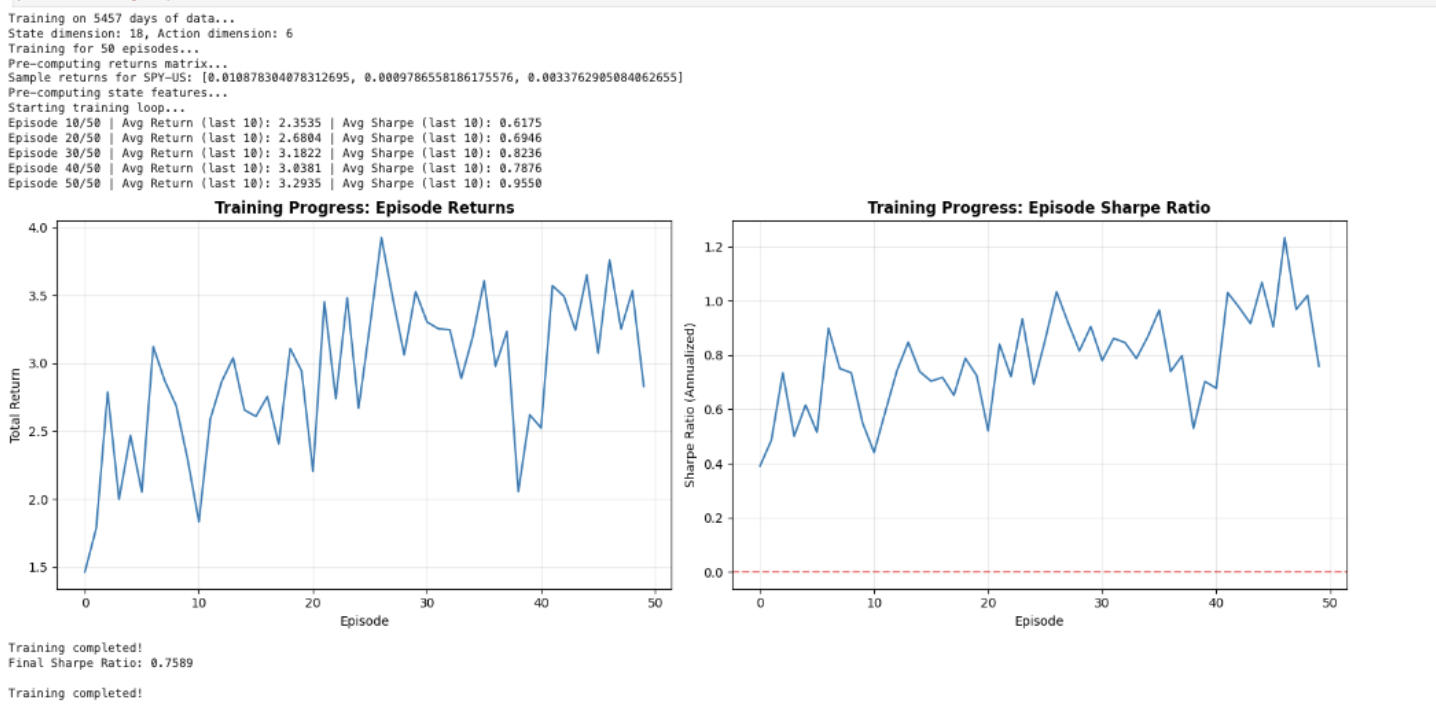
\includegraphics[width=0.85\textwidth]{a.png}
\caption{Average reward, policy loss, and value loss over 50 training epochs.}
\end{figure}
\end{frame}

% ─── Backtest Comparison ─────────────────────────────────────────────────────
\begin{frame}{Backtest: RL vs.\ Equal-Weight Baseline}
\begin{figure}
\centering
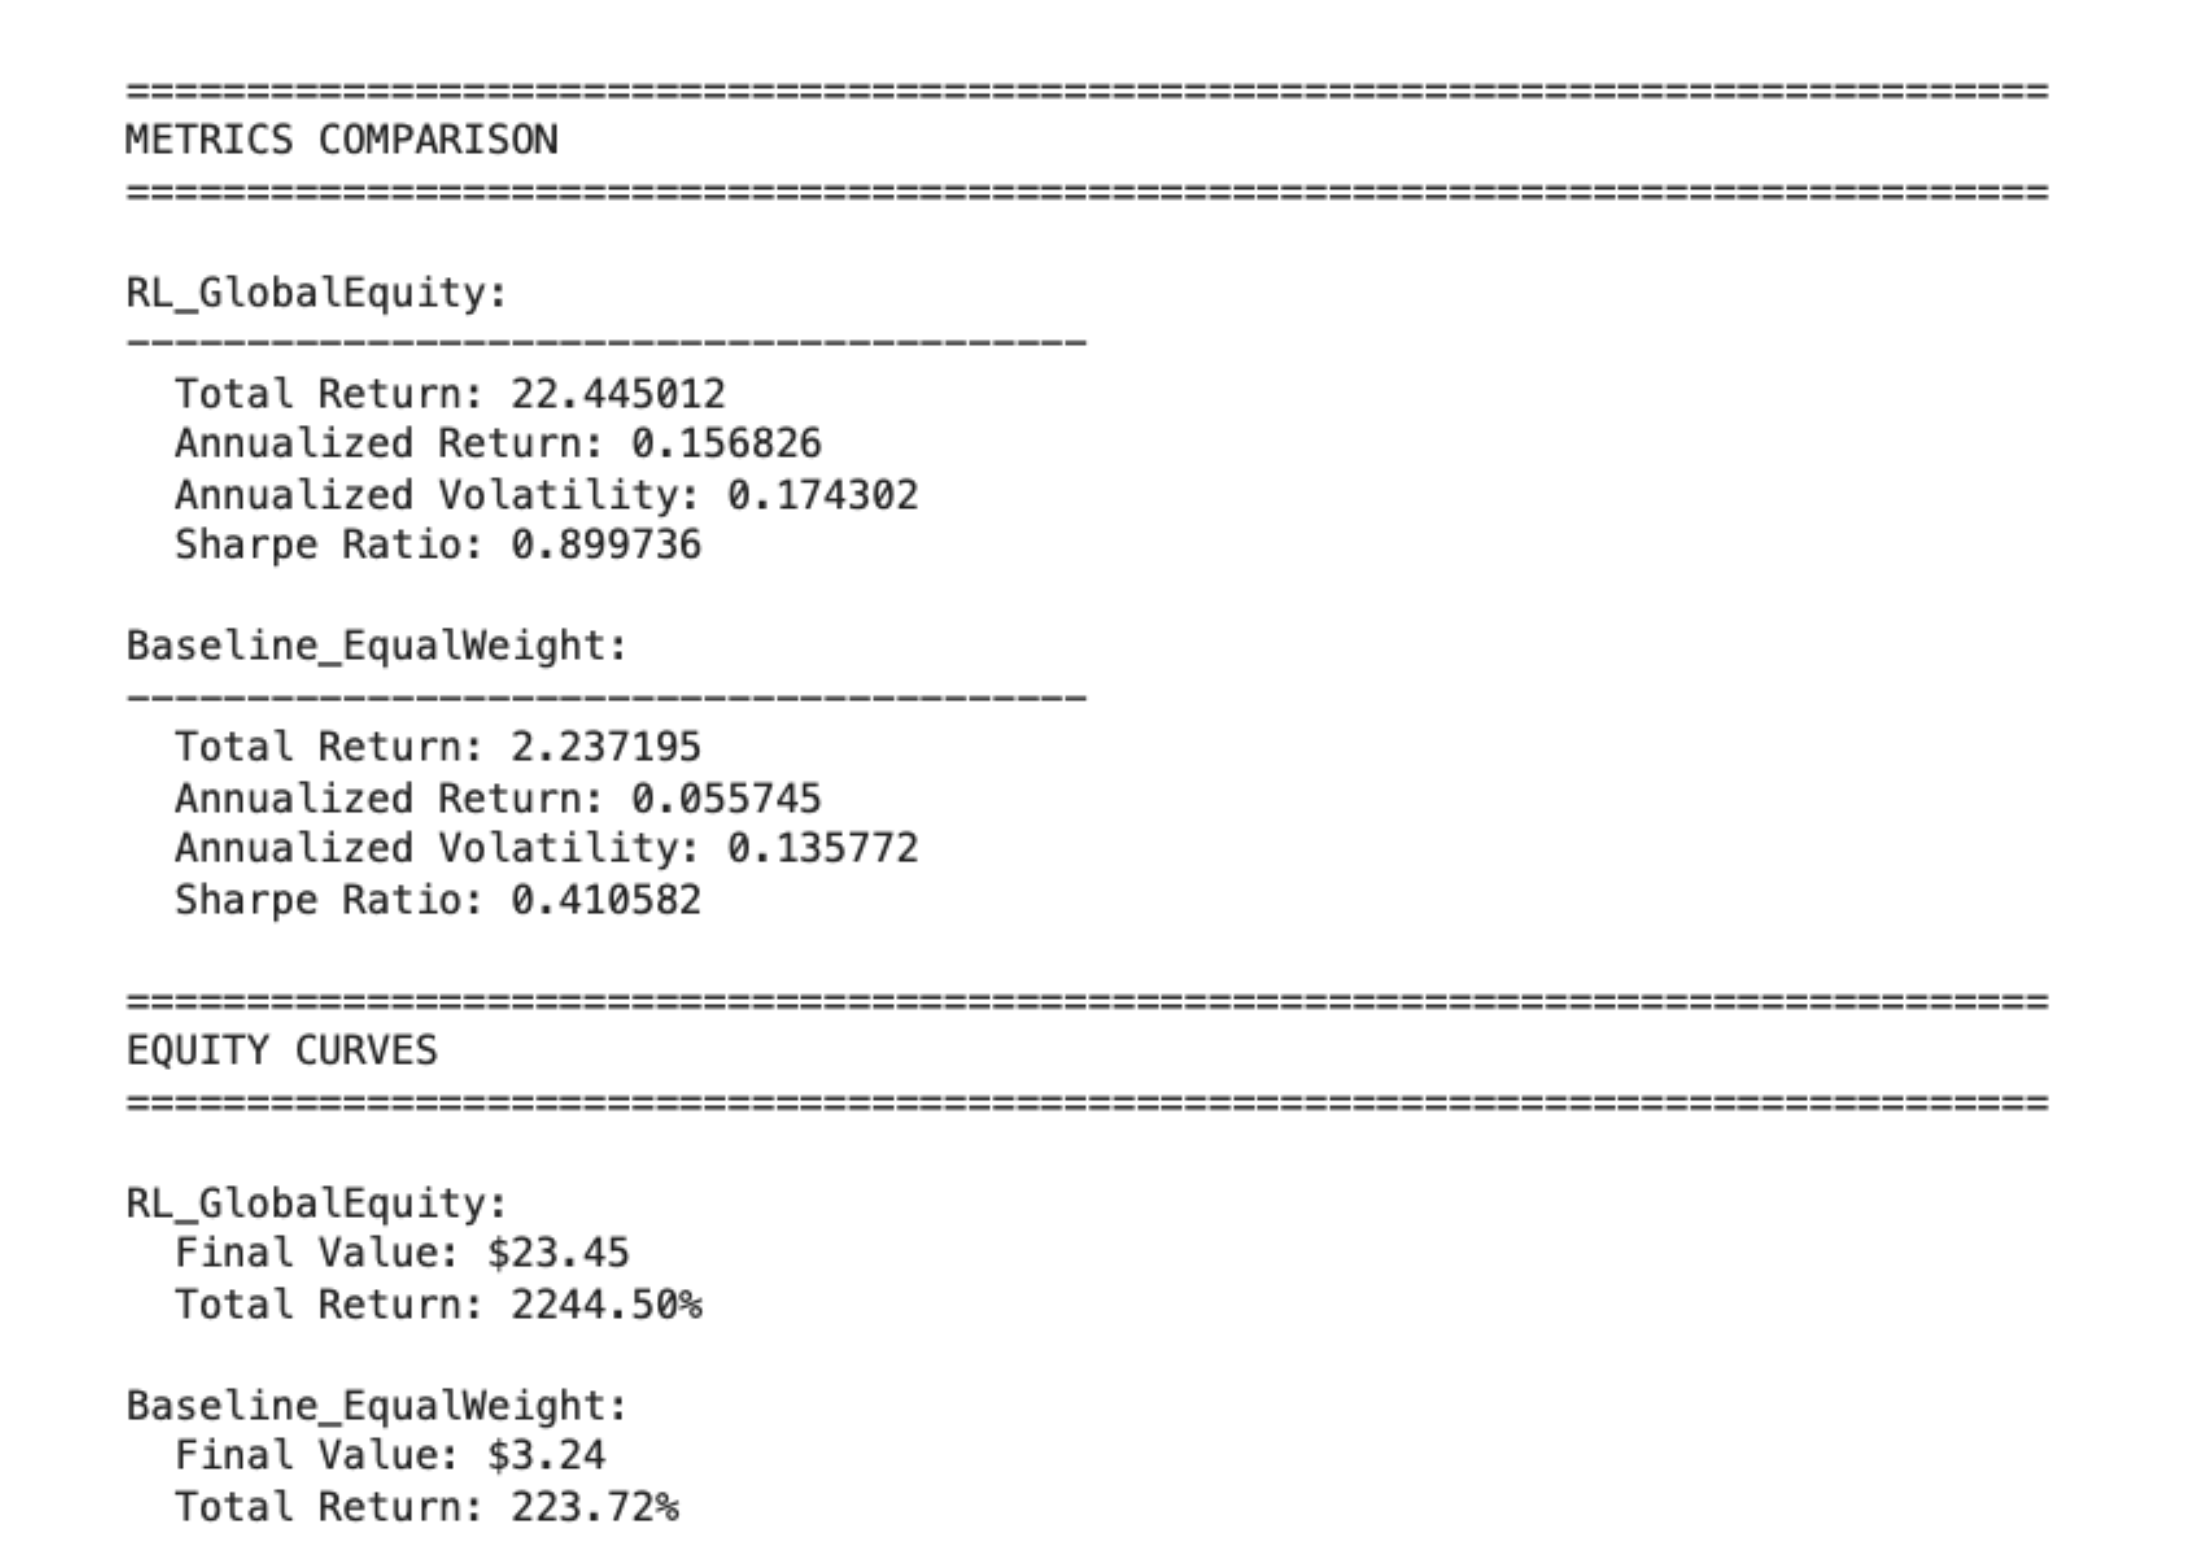
\includegraphics[width=0.85\textwidth]{d.png}
\caption{Performance comparison across training and test periods.}
\end{figure}
\end{frame}

% ─── Equity Curves ───────────────────────────────────────────────────────────
\begin{frame}{Equity Curves}
\begin{figure}
\centering
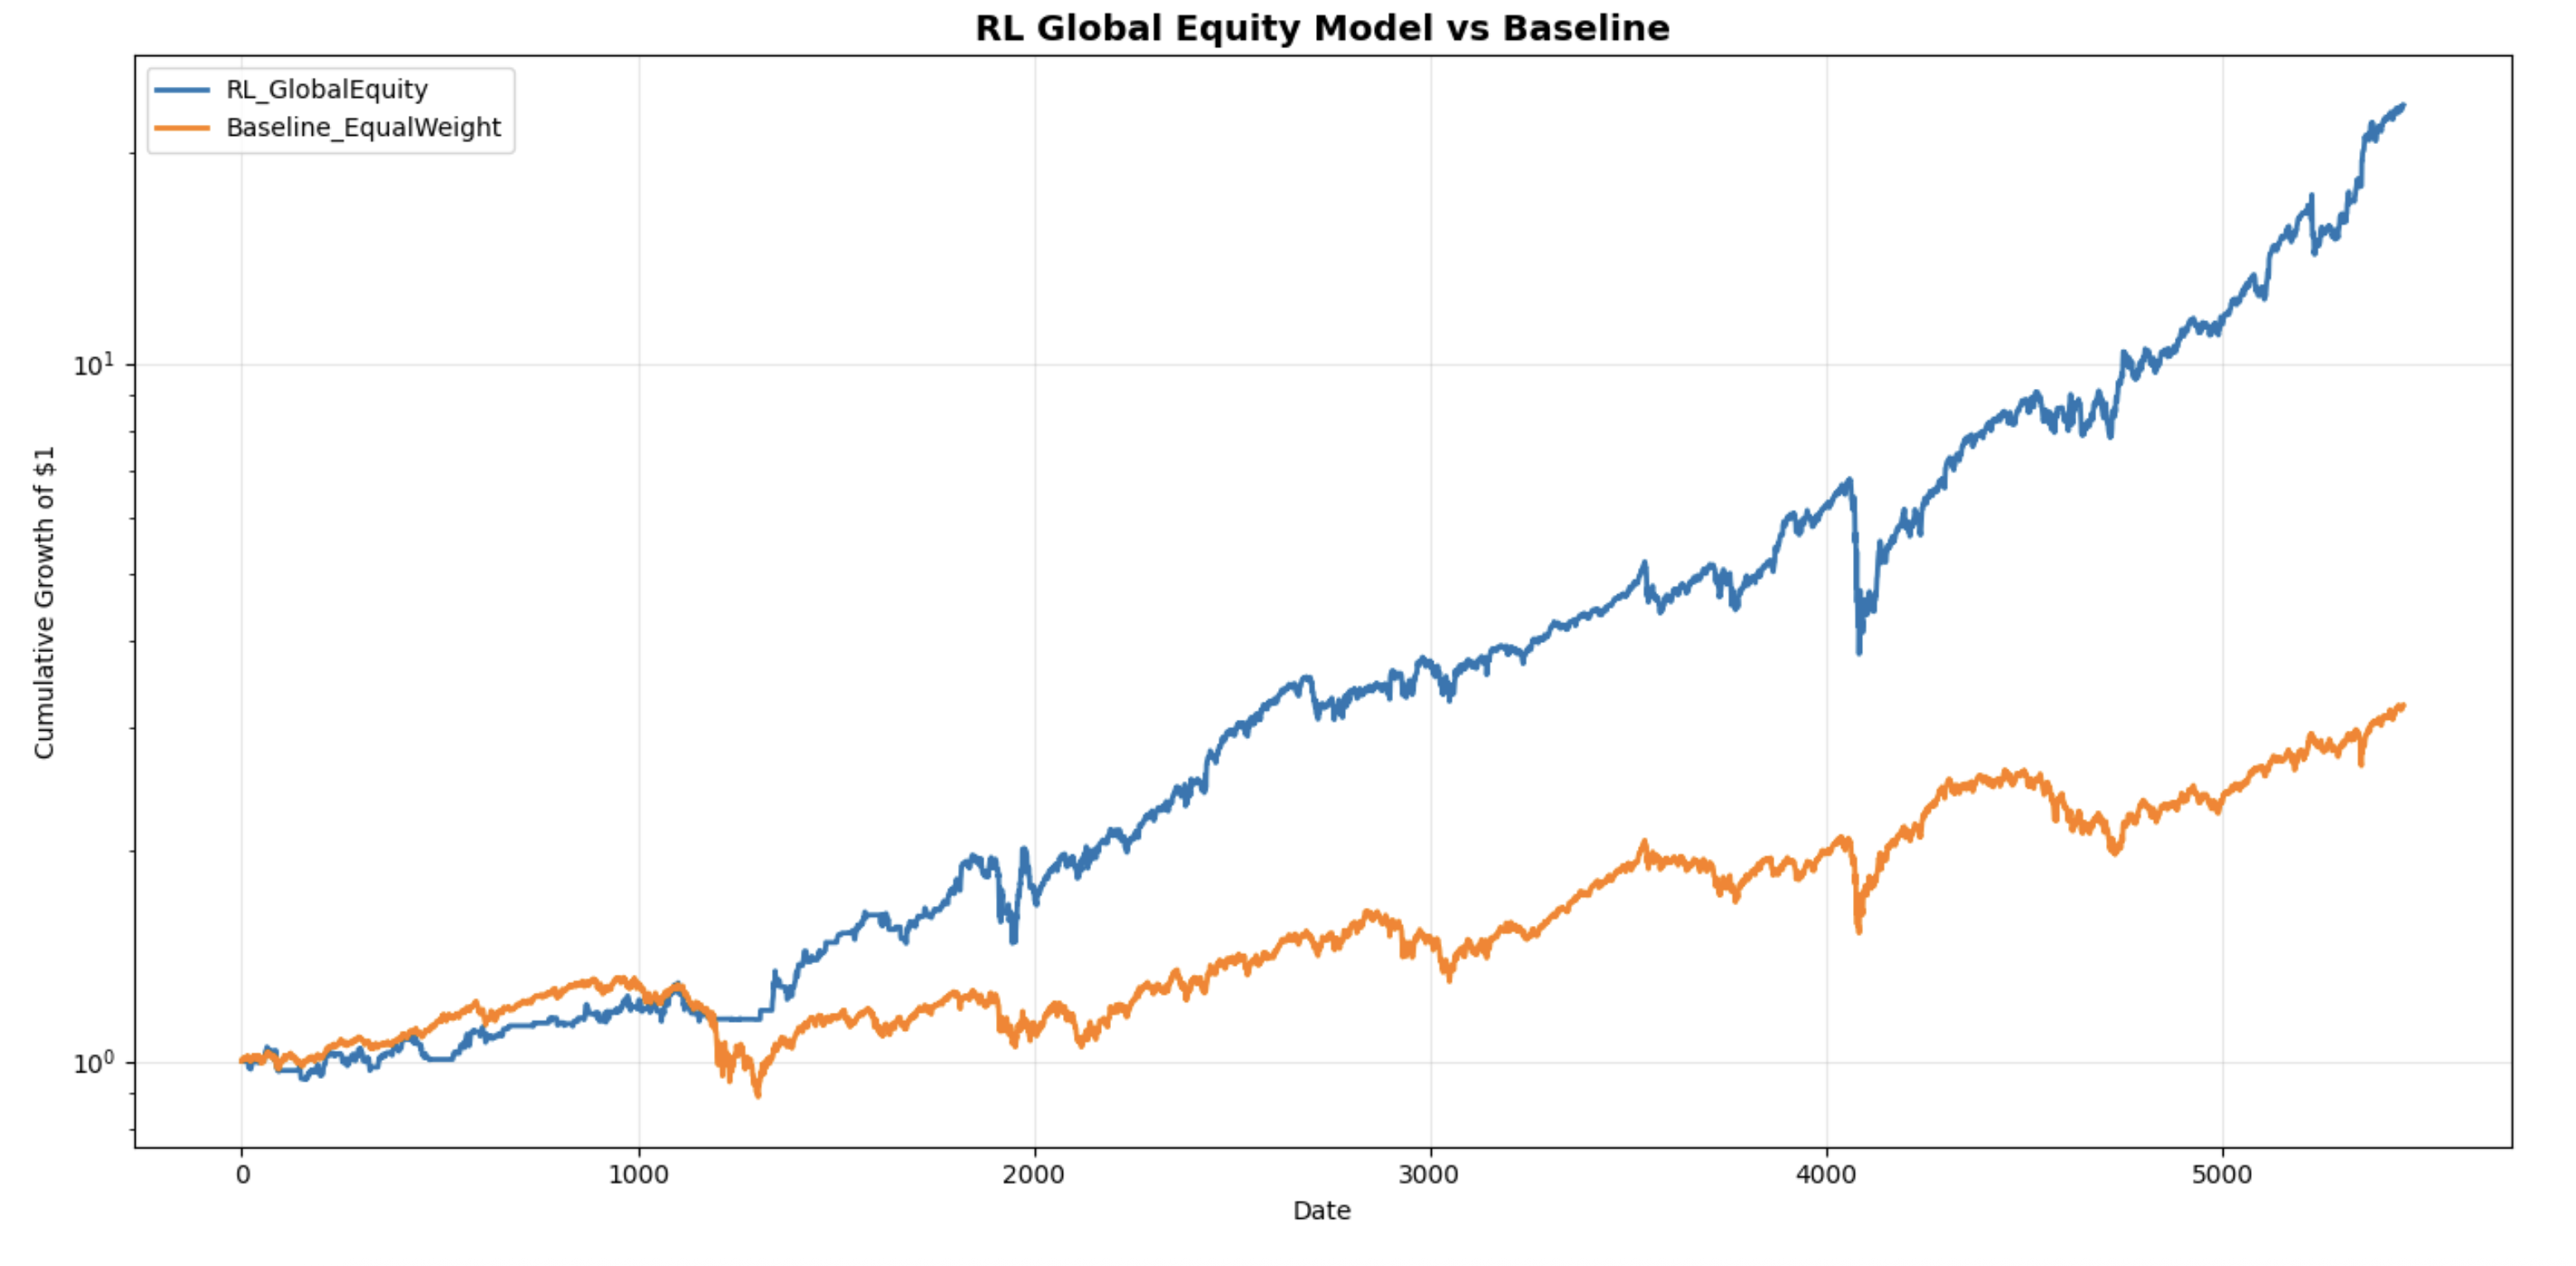
\includegraphics[width=0.85\textwidth]{e.png}
\caption{Cumulative growth of \$1 --- RL model vs.\ equal-weight baseline.}
\end{figure}
\end{frame}

% ─── Key Findings ────────────────────────────────────────────────────────────
\begin{frame}{Key Findings}
\begin{itemize}
    \setlength\itemsep{0.8em}
    \item \textbf{Improved risk-adjusted returns} vs.\ static equal-weight allocation
    \item \textbf{Regime-adaptive} --- rotates between regions and cash based on macro \texttt{bmom}
    \item \textbf{Out-of-sample generalisation} on 2022--2025 test set
    \item \textbf{Blended momentum} reduces state dim from 18 $\to$ 6 without sacrificing signal quality
    \item \textbf{Learned rules} (examples):
        \begin{itemize}
            \item Positive commodity \texttt{bmom} $\Rightarrow$ EWJ-US, EZU-US
            \item Positive VIXY \texttt{bmom} $\Rightarrow$ BIL-US (cash)
            \item Stable macro signals $\Rightarrow$ SPY-US
        \end{itemize}
\end{itemize}
\end{frame}

% ─── Summary ─────────────────────────────────────────────────────────────────
\begin{frame}{Summary}

\begin{columns}[T]
\column{0.5\textwidth}
\textbf{What we built}
\begin{itemize}
    \item PPO-based macro rotation model
    \item Blended momentum state (\texttt{bmom})
    \item 6-asset discrete action space
    \item Risk-penalised reward ($\lambda=0.5$)
\end{itemize}

\column{0.5\textwidth}
\textbf{What we found}
\begin{itemize}
    \item RL learns meaningful macro regimes
    \item \texttt{bmom} weights improve stability
    \item Outperforms equal-weight baseline
    \item Generalises out-of-sample
\end{itemize}
\end{columns}

\bigskip\bigskip
\begin{center}
\large\textbf{Questions?}
\end{center}
\end{frame}

\end{document}
